\begin{figure}[ht]
    \centering
    \begin{subfigure}[t]{0.49\textwidth}
        \centering
		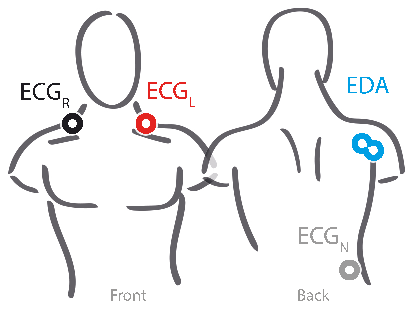
\includegraphics[width=\textwidth]{include/images/electrodes.png}
		\caption{Schematic view of a torso with the placements of the \gls{ECG} and \gls{EDA} electrodes}
        \label{fig:electrodes-schema}
    \end{subfigure}
    \hfill
    \begin{subfigure}[t]{0.49\textwidth}  
        \centering 
		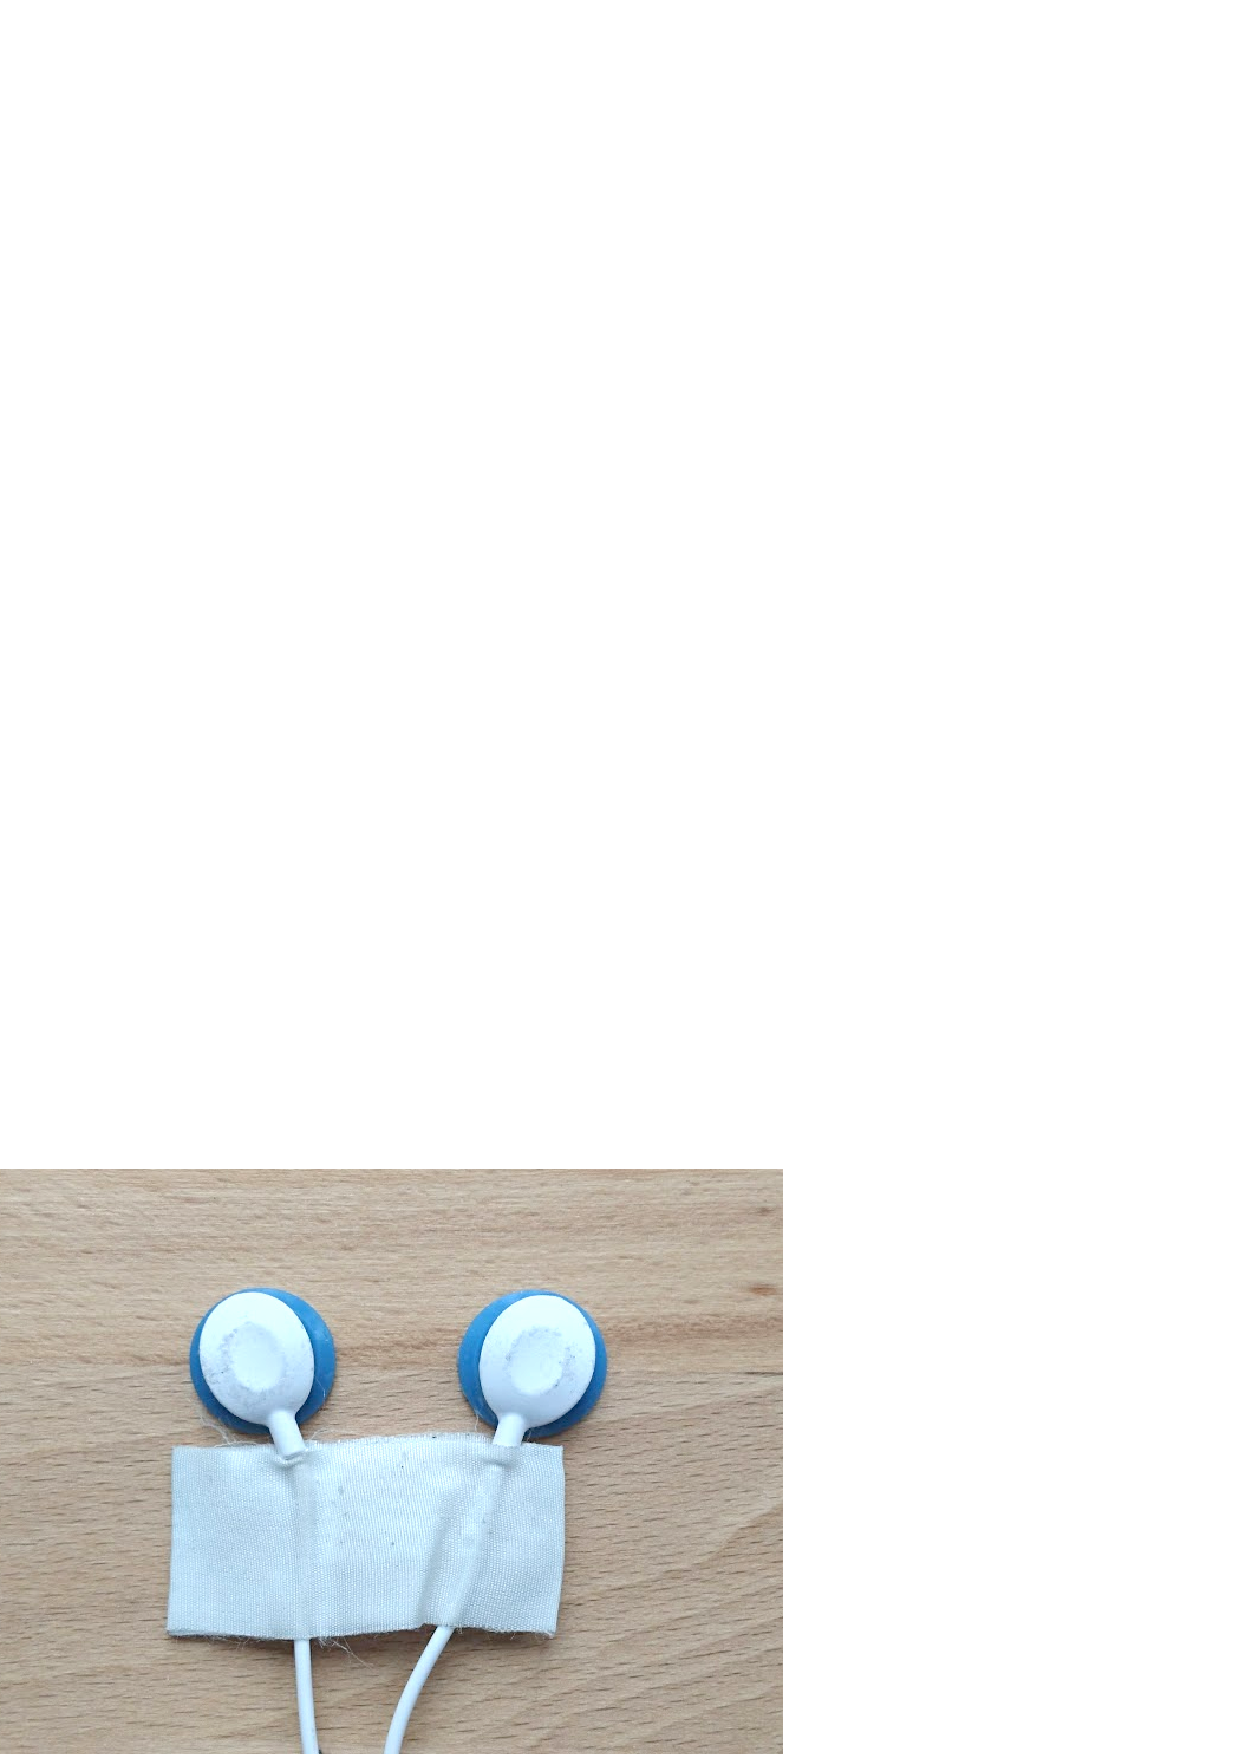
\includegraphics[width=\textwidth]{include/images/electrodes-eda.pdf}
		\caption{\gls{EDA} electrodes prepped with a piece of tape to keep them at a constant distance of \SI{5}{\centi\meter}}
        \label{fig:electrodes-eda}
    \end{subfigure}
    \caption[Placement of electrodes]{Electrodes for \glsfirst{ECG} and \glsfirst{EDA}}
    \label{fig:electrodes}
\end{figure}